\section{About actions}
\labelsec{aboutactions}

In \xss{actions} we said that an \textit{\textbf{action}} is an activity that must always terminate. The effects of an action can be perceived as changes in the logical or in the physical actor environment.

Let us consider here an action that computes the \texttt{n-th} number of Fibonacci (slow, recursive version):

\begin{javacode}
	protected long fibonacci( int n ){
		if( n<0 || n==0 || n == 1 ) return 1;
		else return fibonacci(n-1) + fibonacci(n-2);
	}
\end{javacode}

Usually an action expressed in this way is executed as a procedure that keeps the control until the action is terminated. Since this a 'pure computational action', its effects can be perceived (as a result of type \texttt{long}) when the action returns the control to the caller.


\subsection{Asynchronous Observable Actions}
\labelssec{actionObservable}

Let us introduce now a new idea of an action\footnote{The growing demand for asynchronous, event-driven, parallel and scalable systems demand for new abstractions.} , with the following properties:
\begin{enumerate}
\item the action performs its work in its own thread of control;
\item the action emits an \textit{event} when terminates.
\end{enumerate}

We can define an \textit{\textbf{Observable Action}} is an asynchronous action that emits a termination event\footnote{Usually, the name of the termination event starts with the prefix "\texttt{local\_}", in order to avoid event propagation over the network.}. Moreover:
\begin{itemize}
\item the action can be activated in two different ways: synchronous mode and asynchronous mode;
\item a Observable Action activated in  \textit{synchronous} mode blocks the activator until the action is completed;
\item a Observable Action activated in  \textit{asynchronous} mode returns immediately the control to the activator;
\item the \textit{result} of a Observable Action is an object of some type \texttt{T}.
\end{itemize}

Thus, an Observable Action works in parallel with its activator that can decide to wait for the termination of the action. The action effects (results) can be perceived by means of an operation (if it is defined) that gives (when the action is terminated) the result of the action or by means of an event-driven or an event-based behaviour.

\begin{center}
\begin{tabular}{ c }
     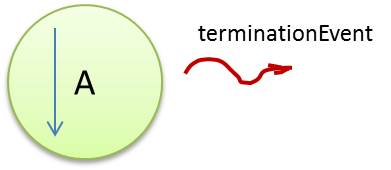
\includegraphics[scale = 0.5]{img/actionObservable.jpg}\\
\end{tabular}{   }
\end{center}
 

\subsection{The class \texttt{ActionObservableGeneric}}
\labelssec{actionObservableGeneric}

The generic, abstract class \texttt{ActionObservableGeneric<T>} provides an implementation support for Observable Actions. It implements the following interface \footnote{The code is included in the file \textit{qactor18.jar}.}  

\lstinputlisting[language=java,caption={ \texttt{IObservableActionGeneric<T>} }, firstline=1 ]{../../../it.unibo.qactor/src/it/unibo/qactors/action/IObservableActionGeneric.java}

The meaning of some important operations is reported in the following table:

\medskip 
\begin{tabular}{|l|l|}
\hline 
\texttt{Future<T> activate()} & starts the action as an asynchronous operation \\ 
\hline 
\texttt{void execAction()} & executes the action and waits for termination \\ 
\hline 
\texttt{long getExecTime()} & returns the execution time of the action \\ 
\hline 
\texttt{String getTerminationEventId()} & returns the name of the termination event\\ 
\hline 
\texttt{String getResultRep()} & returns (a representation of) the result of the action\\ 
\hline 
\end{tabular} 

 

\subsubsection{The interface \texttt{Callable<T>}.\\}
Since an Observable Action is a \texttt{java.util.concurrent.Callable<T>}, it must define the operation \texttt{<T> call()}.
The \texttt{Callable} interface is similar to \texttt{Runnable}, in that both are designed for classes whose instances are potentially executed by another thread. A \texttt{Runnable}, however, \textit{does not return a result} and cannot throw a checked exception.

\subsubsection{The interface \texttt{Future<T>}.\\}
\labelssec{future}

The operation \texttt{activate} starts the execution of the action (see \xss{activate}) and returns an object that must implement the interface \texttt{java.util.concurrent.Future<T>}. 

In \java{}, a \texttt{Future} represents the result of an asynchronous computation. It exposes methods allowing a client to monitor the progress of a task being executed by a different thread. Therefore a Future object can be used to check the status of a \texttt{Callable} and to retrieve the result from the \texttt{Callable}. More specifically:
\begin{itemize}
\item Check whether a task has been completed or not.
\item  Cancel a task.
\item Check whether task was cancelled or complete normally.
\end{itemize}
 
In programming languages, the \textit{future} concept is also known as \textit{promises} or \textit{delays}.


\subsubsection{The operation \texttt{activate}.\\}
\labelssec{activate}

The operation \texttt{activate()} starts the action as an asynchronous operation by using the class \texttt{java.util.concurrent.Executors}
\begin{javacode}
protected Future<T>  fResult;
	public Future<T> activate() throws Exception{
		Result = EventPlatformKb.manyThreadexecutor.submit(this);	
 		return fResult;
 	}
\end{javacode} 

\subsubsection{The class \texttt{Executors}.\\}
\labelssec{future}

Since working with the \texttt{Thread} class can be very tedious and error-prone, the \textit{Concurrency API} has been introduced back in \texttt{2004} with the release of \texttt{Java 5}. The \texttt{API} is located in package \textit{java.util.concurrent} and contains many useful classes for handling concurrent programming, including the concept of an \textit{ExecutorService} as a higher level replacement for working with threads directly. Executors are capable of running asynchronous tasks and typically manage a pool of threads. 

\subsubsection{The operation \texttt{execAction}.\\}
\labelssec{execAction}

The operation \texttt{execAction()} activates the action and forces the caller to waits for the termination of the action execution.

\begin{javacode}
	@Override
	public void execAction() throws Exception {
		activate();
		fResult.get();	//to force the caller to wait
	}
\end{javacode}



\subsubsection{The operation \texttt{T call}.\\}
\labelssec{call}

The operation \texttt{T call()} is the entry point for the Executor and is defined as a sequence of internal operations that starts by taking the current time and ends by calculating the execution time and by emitting the action termination event.

\begin{javacode}
	/* Entry point for the Executor */
	@Override
	public T call() throws Exception {
		startOfAction(); 
		execTheAction();
		result = endActionInternal();
		return result;
	}
\end{javacode}

\subsubsection{The operation \texttt{startOfAction}.\\}
\labelssec{startOfAction} 

The operation \texttt{startOfAction} takes the current time and retains a reference to the current Thread:
\begin{javacode}
protected Thread myself;
	protected void startOfAction() throws Exception{
		tStart = Calendar.getInstance().getTimeInMillis();
		myself = Thread.currentThread();		
	}
\end{javacode}

\subsubsection{The operation \texttt{endActionInternal}.\\}
\labelssec{endActionInternal} is executed when the action is terminated; it evaluates the action execution time and emits the termination event with payload \texttt{result(RES,EXECTIME)}:

The operation \texttt{endActionInternal} 
\begin{javacode}
 	/* Calculate action execution time and emit the termination event */
	protected T endActionInternal() throws Exception{
 		T res = endOfAction();
		emitEvent( terminationEvId, res );
		return res;
	}
	protected void emitEvent(String event, T res){
		long tEnd = Calendar.getInstance().getTimeInMillis();
		durationMillis =  tEnd - tStart ;	
    	platform.raiseEvent( getName(), event, "result("+res+",exectime("+durationMillis+"))" );		
	} 
\end{javacode}

\subsubsection{The operations \texttt{execTheAction} and  \texttt{endOfAction }.\\}
The operations \texttt{execTheAction} and \texttt{endOfAction} are declared \texttt{abstract} in the class \textit{ActionObservableGeneric<T>}. 

\begin{javacode}
	/* TO BE DEFINED BY THE APPLICATION DESIGNER */
	protected abstract void execTheAction() throws Exception; 
	protected abstract T endOfAction() throws Exception; 
\end{javacode}

These operations must be defined by the application designer in the following way:

\medskip 
\begin{tabular}{|l|l|}
\hline 
\texttt{execTheAction} & defines the 'businnes logic' of the action \\ 
\hline 
\texttt{endOfAction} & returns the main result of the action \\ 
\hline 
\end{tabular} 
 
\subsection{Fibonacci as Observable Action}
The \texttt{fibonacci} computation of \xs{aboutactions} is defined in the following as a Observable Action that takes at construction time a goal of the form \texttt{fibo(N,V)} where \texttt{N} is the fibonacci number to evaluate and \texttt{V} is the (variable that denotes the) result

\lstinputlisting[language=java,caption={ \texttt{ActionObservableFibonacci<T>} }, firstline=1 ]{../../../it.unibo.robot.interactive/src/it/unibo/actionobsexecutor/ActionObservableFibonacci.java}

\subsubsection{Experiments on Fibonacci as Observable Action.}

The project \textit{it.unibo.robot.interactive}, package \texttt{it.unibo.actionobsexecutor} shows the effects of the action in the different execution modes:



\begin{center}
\begin{tabular}{ c }
     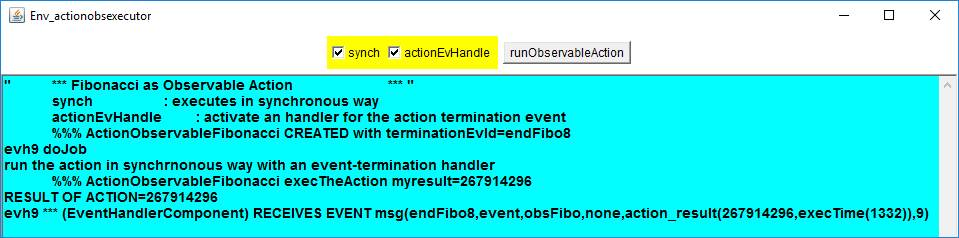
\includegraphics[scale = 0.6]{img/actionObs.jpg}\\
\end{tabular}{   }
\end{center}


 \newpage 
\subsection{Timed actions}
\labelssec{timedAction}

In several situations, an application designer could activate actions that must always terminate within a prefixed amount of time. In \xss{planactions} we have introduced the idea of \textit{timed action}.

We can define an \textit{\textbf{Timed Action}} as an \textit{Observable Action} whose execution time \texttt{T} satisfies the constraint \texttt{T<=DURATION}, where \texttt{DURATION} is a prefixed amount of time\footnote{Usually, \texttt{T} and \texttt{DURATION} are expressed in millisecs.}. Moreover:
\begin{itemize}
\item the action can be activated in two different ways: \textit{synchronous mode} and \textit{asynchronous mode};
\item a Timed Action activated in  \textit{\textbf{synchronous}} mode: \textit{i)} blocks the activator until the action is completed and \textit{ii)} emits a termination event when it ends its work;
\item a Timed Action activated in  \textit{\textbf{asynchronous}} mode:  \textit{i)} returns immediately the control to the activator, \textit{ii)} emits immediately the termination event and \textit{iii)} emits another event (called \textit{\textbf{answer} event}) when it ends its work;
\item a Timed Action can be \textit{\textbf{suspended}} (interrupted) even if it not already terminated. A Timed Action is called \textbf{\textit{recoverable}} if the action can resume its work after a suspension.
\item the \textit{\textbf{result}} of a Timed Action is an object (of type \texttt{AsynchActionGenericResult<T>}, see \xss{AsynchActionGenericResult}) that the wraps the application result into a structure that gives other information about the action (e.g. interrupted or not, execution time remained with respect to the \texttt{DURATION}, etc.)
 \item 
\end{itemize}

Thus, a Timed Action works in its own thread of control; its activator can decide to wait for the termination of the action (\textit{synchronous mode} activation) or to continue its work. In case of \textit{asynchronous mode} activation, an actor interested in the application result of the action can look at the \textit{answer event} emitted by the action. An actor can also suspend an action, and, if the action is recoverable, continue its execution later\footnote{This kind of behaviour is useful for example  when a robot must execute a move for some time, while being able to reacts to alarms.}. 

\subsection{The class \texttt{ActorTimedAction}}
\labelssec{ActorAction} 
The class \texttt{ActorTimedAction} implements the concept of Timed Action by building a 'subsystem' composed of the action and other two components: a timer and a event handler:

%and is the basic building block for the different types of \textit{PlanActions} introduced in \xss{planactions}:

\medskip 
\begin{center}
\medskip 
\begin{tabular}{|c|c|}
\hline 
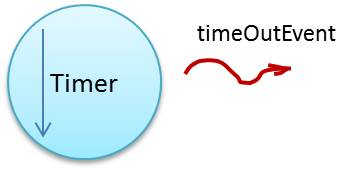
\includegraphics[scale = 0.5]{img/actionTimer.jpg} & 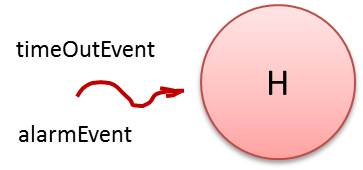
\includegraphics[scale = 0.5]{img/actionEventHandler.jpg} \\ 
\hline 
\end{tabular}
\end{center}

\lstinputlisting[language=java,caption={ \texttt{ActorTimedAction} }, firstline=1 ]{../../../it.unibo.qactor/src/it/unibo/qactors/action/ActorTimedAction.java}

The architecture of the 'subsystem' built by the \texttt{init} operation of \texttt{ActorAction} is shown in the following picture:

\begin{center}
\begin{tabular}{ c }
     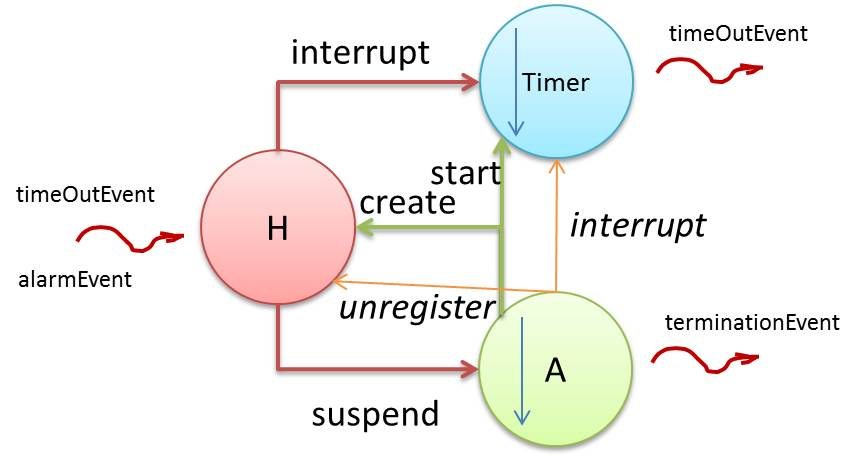
\includegraphics[scale = 0.5]{img/actionTimedReactive.jpg}\\
\end{tabular}{   }
\end{center}




\subsection{The class \texttt{AsynchActionGeneric}}
\labelssec{AsynchActionGeneric}

The generic, abstract class \texttt{AsynchActionGeneric<T>} provides the \texttt{API} for Timed Actions, as defined by the following interface \footnote{The code is included in the file \textit{qactor18.jar}.}  

\lstinputlisting[language=java,caption={ \texttt{IAsynchAction<T>} }, firstline=1 ]{../../../it.unibo.qactor/src/it/unibo/qactors/action/IAsynchAction.java}

The meaning of some important operations is reported in the following table:

\medskip 
\noindent
\begin{scriptsize}
\begin{tabular}{|l|l|}
\hline 
\texttt{AsynchActionGenericResult<T> execSynch()} & executes the action in synchronous way (waits for termination) \\ 
\hline 
\texttt{Future<AsynchActionGenericResult<T>> execAsynch} & executes the action in asynchronous way \\ 
\hline 
\texttt{AsynchActionGenericResult<T> waitForTermination()} & waits until the action is terminated (mainly for execAsynch) \\ 
\hline 
\texttt{void suspendAction()} & suspends the execution of the action if not already terminated \\ 
\hline 
\texttt{ActionRunMode getExecMode()} & returns an instance of ActionRunMode (termination with answer or not) \\  
\hline 
\end{tabular} 
\end{scriptsize}  

\subsection{The class \texttt{AsynchActionGenericResult}}
\labelssec{AsynchActionGenericResult}

The generic class \texttt{AsynchActionGenericResult<T>} provides objects that represent the result of a Timed Action:

\lstinputlisting[language=java,caption={ \texttt{AsynchActionGenericResult<T>} }, firstline=1  ]{../../../it.unibo.qactor/src/it/unibo/qactors/action/AsynchActionGenericResult.java}


\subsection{Fibonacci as a Timed Action}
\labelssec{fibotimed}

The \texttt{fibonacci} computation of \xs{aboutactions} is defined in the following as a Timed Action that takes at construction time a goal of the form \texttt{fibo(N,V)} where \texttt{N} is the fibonacci number to evaluate and \texttt{V} is the (variable that denotes the) result.

\lstinputlisting[language=java,caption={ \texttt{ActionTimedFibonacci<T>} }, firstline=1 ]{../../../it.unibo.robot.interactive/src/it/unibo/actiontimedexecutor/ActionTimedFibonacci.java}

\subsubsection{Experiments on Fibonacci as Timed Action.}

The Project \textit{it.unibo.robot.interactive}, package \texttt{it.unibo.actiontimedexecutor} shows the effects of the action in the different execution modes:
 
\begin{center}
\begin{tabular}{ c }
     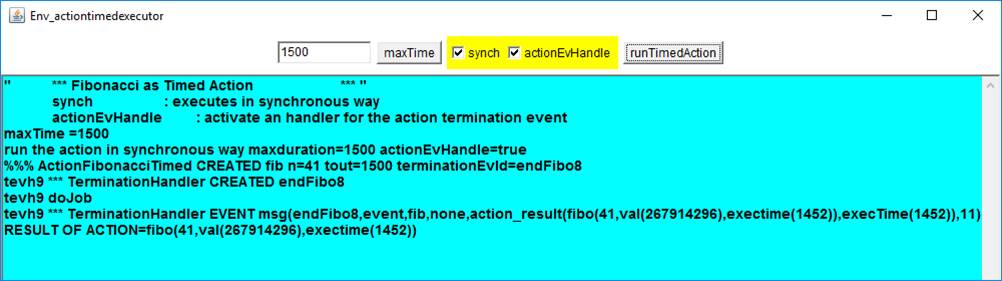
\includegraphics[scale = 0.6]{img/actionTimed.jpg}\\
\end{tabular} 
\end{center}



 \newpage 
\subsection{Reactive actions}
\labelssec{reactiveactions}
We can define a \textit{\textbf{Reactive Action}} as a \textit{Timed Action} that can be suspended (interrupted) by the occurrence of events.  

The occurrence of an event E that suspends the execution of a reactive action RA in a plan P, gives raise to the execution of a plan EP associated to the event E. The plan EP, once terminated, can terminate the behaviour of the Actor or resume the plan P, that will be continue from the suspension point of the action RA, if it is recoverable, or from the action that follows RA in P.

%% The execution of a Reactive Action is done under the control of a \textit{TaskActionFsmExecutor} that is able to handle the action termination-event and any expected 'interruption' event (including a time-out) that can happen while the action is running. 

%%This Reactive Action executor is a specialization of an abstract \texttt{TaskComponent} that implements a event-based finite-state machine whose input-set is called \textit{inputSymbolEventsSet}. The run-time support resumes a Task only when the current event belongs to \textit{inputSymbolEventsSet} and this input is in the \textit{expectedInput} set of its current Task \textit{state}. This work is done by an event handler (of class \textit{TaskQueueEventHandler}) that:
%% \begin{itemize}
%% \item is automatically created when a new Task instance is created
%% \item reacts to all the events that belong to the  \textit{inputSymbolEventsSet} of the Task;
%% \item resumes the Task if it is not already activated;
%% \item stores the event in a local queue if the Task already activated.
%% \end{itemize}

 

\subsection{Fibonacci as a Reactive Action}
\labelsec{fiboreactive}

 
The \texttt{fibonacci} computation of \xss{fibotimed} can be used to build a Reactive Action, by introducing a test to 'interrupt' the action if it has been suspended by some event.

\lstinputlisting[language=java,caption={ \texttt{ActionReactiveFibonacci<T>} }, firstline=1 ]{../../../it.unibo.robot.interactive/src/it/unibo/actionreactiveexecutor/ActionReactiveFibonacci.java}

\subsubsection{Experiments on Fibonacci as Reactive Action.}

The Project \textit{it.unibo.robot.interactive}, package \texttt{it.unibo.actionreactiveexecutor} shows the effects of the action in the different execution modes. When the \texttt{interrupt} flag is set, an event \texttt{usercnd : stop} is generated\footnote{The \texttt{QActor} operation \texttt{emitEventAsynch} performs the task to generate a given event after a given time.} after \texttt{maxtime/2} \textit{msecs}. 


\begin{center}
\begin{tabular}{ c }
     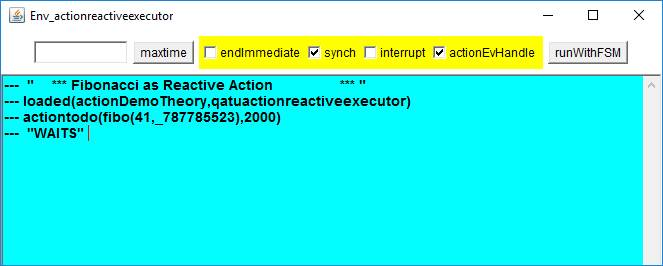
\includegraphics[scale = 0.6]{img/actionReactive.jpg}\\
\end{tabular} 
\end{center}
